\section{Capítulo 2: Marco teórico}

En este capítulo se presentan los fundamentos teóricos que sustentan el desarrollo del proyecto, abordando tanto los aspectos pedagógicos relacionados con la adquisición de la escritura en educación primaria como los elementos tecnológicos que permiten su análisis automatizado. Se revisan conceptos vinculados al proceso de consolidación de la ortografía y la calidad del trazo manuscrito, así como los principios básicos del OCR, el NLP y la arquitectura de sistemas web. El propósito de este marco teórico es proporcionar el sustento conceptual necesario para comprender la propuesta planteada y establecer la base académica sobre la cual se desarrolla la solución tecnológica.

\subsection{Fundamentos de la escritura en la educación}

La escritura en educación primaria constituye una habilidad esencial para el desarrollo académico y social de los estudiantes. La alfabetización temprana permite que los niños adquieran competencias básicas de lectura y escritura que influyen directamente en su capacidad de aprendizaje a lo largo de la trayectoria escolar \cite{unesco2024aprendizajes}. El dominio de estas habilidades no solo impacta el área de lenguaje, sino que favorece el desempeño en otras disciplinas al facilitar la comprensión y expresión de ideas, así como el desarrollo de habilidades comunicativas fundamentales.

Organismos internacionales han señalado que fortalecer la lectura y escritura desde los primeros grados escolares contribuye significativamente a mejorar los resultados educativos y reducir brechas de aprendizaje \cite{unesco2024alfabetizacion}. En este sentido, la escritura no se limita a la producción mecánica de palabras, sino que implica procesos cognitivos complejos relacionados con la organización del pensamiento, la memoria y la estructuración de ideas. Estos procesos permiten al estudiante no solo reproducir información, sino también interpretarla, analizarla y expresarla de manera coherente.

La práctica de la escritura manuscrita desempeña un papel relevante en este proceso, ya que favorece la coordinación motora fina y la consolidación de la relación entre grafemas y fonemas. Diversos recursos educativos destacan que la enseñanza explícita de la escritura a mano fortalece la identificación de letras, la ortografía y la retención de información \cite{readingrockets2024importance}. Asimismo, la escritura activa múltiples procesos cognitivos vinculados con la atención, la memoria de trabajo y el aprendizaje significativo, lo que contribuye a una mayor internalización del conocimiento \cite{edutopia2024teaching}.

Además, el desarrollo de la escritura en esta etapa implica la interacción de distintos factores que van más allá del aspecto lingüístico, incluyendo habilidades motoras, cognitivas y pedagógicas. La integración de estos elementos permite que el estudiante desarrolle progresivamente la capacidad de expresar ideas de manera clara, estructurada y coherente, lo cual es fundamental para su desempeño académico.

En este sentido, el desarrollo de la escritura en educación primaria puede entenderse como un proceso integral que combina aspectos lingüísticos, cognitivos y motrices. La identificación de sus componentes fundamentales permite establecer criterios claros para su evaluación y fortalecimiento dentro de entornos educativos formales. Como se presenta en la Tabla \ref{tab:componentes}, dichos componentes permiten comprender de manera estructurada los elementos que influyen directamente en el aprendizaje de la escritura.


\begin{longtable}{|p{3.5cm}|p{5cm}|p{4.5cm}|}
\caption{Componentes de la escritura y su impacto en el aprendizaje.}
\label{tab:componentes} \\

\hline
\textbf{Componente} & 
\textbf{Descripción} & 
\textbf{Impacto en el aprendizaje} \\
\hline
\endfirsthead

\hline
\textbf{Componente} & 
\textbf{Descripción} & 
\textbf{Impacto en el aprendizaje} \\
\hline
\endhead

\hline
\endfoot

Motricidad fina & Coordinación y control del trazo manuscrito & Mejora la legibilidad \\
\hline

Ortografía & Aplicación correcta de reglas lingüísticas & Favorece claridad textual \\
\hline

Conciencia fonológica & Relación entre sonidos y grafías & Reduce errores frecuentes \\
\hline

Organización escrita & Estructuración coherente de ideas & Facilita comprensión \\
\hline

Retroalimentación & Corrección continua del desempeño & Refuerza el aprendizaje \\
\hline

\end{longtable}

\subsection{Alfabetización digital en entornos educativos}

La alfabetización digital se refiere a la capacidad de utilizar tecnologías de la información y la comunicación de manera efectiva, crítica y responsable dentro de distintos contextos, incluido el educativo. En los últimos años, organismos internacionales han destacado la necesidad de integrar herramientas digitales como parte complementaria del proceso de enseñanza-aprendizaje, especialmente en educación básica \cite{unesco2024digitallit}. Esta integración no solo implica el uso de dispositivos tecnológicos, sino también el desarrollo de competencias que permitan a los estudiantes interactuar con la información de manera reflexiva y autónoma.

La incorporación de tecnología en el aula no implica sustituir la función del docente, sino ampliar las posibilidades de retroalimentación, seguimiento y acceso a recursos educativos. La Organización de las Naciones Unidas para la Educación, la Ciencia y la Cultura (United Nations Educational, Scientific and Cultural Organization, UNESCO por sus siglas en inglés) ha señalado que el uso adecuado de tecnologías digitales puede fortalecer competencias fundamentales cuando se implementa bajo criterios pedagógicos claros \cite{unesco2021ai}. Asimismo, el Banco Mundial ha subrayado que las soluciones tecnológicas en educación deben diseñarse con un enfoque centrado en el aprendizaje y no únicamente en la herramienta tecnológica \cite{worldbank2023reimagining}. Esto implica que el valor de la tecnología radica en su correcta integración dentro de estrategias didácticas bien estructuradas.

En el caso de la escritura, muchas plataformas digitales actuales se enfocan en ejercicios mecanografiados, dejando en segundo plano la práctica manuscrita. Esta situación evidencia la necesidad de explorar propuestas que integren tecnología sin abandonar habilidades tradicionales esenciales. La alfabetización digital, por tanto, no consiste únicamente en el uso de dispositivos, sino en la integración estratégica de herramientas que potencien el aprendizaje significativo y mantengan un equilibrio entre lo digital y lo manual.
Además, es importante considerar que la implementación de tecnologías en entornos educativos conlleva tanto beneficios como retos, los cuales deben ser analizados para garantizar un uso adecuado. Factores como la infraestructura tecnológica, la capacitación docente y el acceso equitativo a los recursos influyen directamente en el impacto de estas herramientas dentro del proceso educativo.

Las principales ventajas y desafíos asociados al uso de tecnología en educación básica se presentan en la Tabla \ref{tab:ventajas}, donde se sintetizan los elementos más relevantes que intervienen en la integración tecnológica dentro del aula.

\begin{longtable}{|p{6cm}|p{7cm}|}
\caption{Ventajas y desafíos de la integración tecnológica en educación básica.}
\label{tab:ventajas} \\

\hline
\textbf{Aspecto} & \textbf{Descripción} \\
\hline
\endfirsthead

\hline
\textbf{Aspecto} & \textbf{Descripción} \\
\hline
\endhead

\hline
\endfoot

Retroalimentación inmediata & Permite correcciones en tiempo real \\
\hline

Seguimiento individualizado & Facilita monitoreo del progreso \\
\hline

Motivación del estudiante & Incrementa interés y participación \\
\hline

Dependencia tecnológica & Requiere infraestructura adecuada \\
\hline

Brecha digital & Puede generar desigualdades de acceso \\
\hline

\end{longtable}

El análisis de estos factores permite comprender que la tecnología, cuando se implementa como herramienta complementaria y supervisada, puede contribuir significativamente al fortalecimiento de competencias académicas fundamentales, favoreciendo tanto el aprendizaje individual como el desarrollo de habilidades digitales necesarias en el contexto actual.

\subsection{OCR}

El OCR es una tecnología que permite convertir imágenes que contienen texto impreso o manuscrito en información digital procesable por un sistema computacional \cite{smith2007overview}. Su aplicación se ha extendido en distintos ámbitos, como la digitalización de documentos, la automatización de formularios y el procesamiento de información textual a partir de imágenes escaneadas, facilitando la gestión y análisis de grandes volúmenes de información.

El funcionamiento del OCR se basa en una serie de etapas secuenciales que permiten transformar la imagen original en texto estructurado. De manera general, el proceso inicia con la adquisición de una imagen que contiene caracteres y continúa con procedimientos de análisis y reconocimiento automatizado, los cuales permiten interpretar la información visual de forma sistemática.
En la Figura \ref{fig:OCR} se presenta el flujo general del proceso OCR, el cual describe las etapas principales involucradas en la transformación de una imagen en texto digital.

\begin{figure}[H]
    \centering
    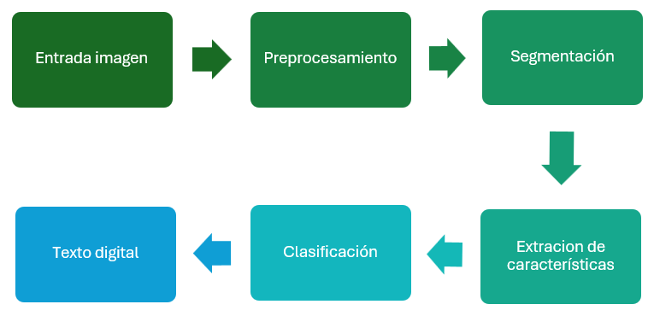
\includegraphics[width=0.7\textwidth]{Imagenes/procesoOCR.png}
    \caption{Flujo general del proceso OCR adaptado.}
    \label{fig:OCR}
\end{figure}
Adaptado de \cite{otsu1979threshold, smith2007overview}

Como se observa en la Figura \ref{fig:OCR}, el proceso comienza con la entrada de una imagen, que puede provenir de una fotografía o de un lienzo digital. Posteriormente, en la etapa de preprocesamiento, se realizan ajustes como conversión a escala de grises, binarización y eliminación de ruido, con el fin de mejorar la calidad visual para su análisis \cite{otsu1979threshold}. Estas técnicas permiten reducir variaciones no deseadas en la imagen, facilitando el reconocimiento posterior de los caracteres.

En la fase de segmentación, el sistema identifica y separa los caracteres individuales o grupos de caracteres dentro de la imagen. Este proceso resulta crítico, ya que una segmentación incorrecta puede afectar directamente la precisión del reconocimiento. A continuación, durante la extracción de características, se analizan propiedades específicas como contornos, formas y patrones estructurales que permiten diferenciar un carácter de otro.

Finalmente, en la etapa de clasificación, el sistema compara las características extraídas con modelos previamente entrenados para determinar a qué carácter corresponde cada patrón identificado, generando como resultado el texto digital final \cite{smith2007overview}. Esta etapa constituye el núcleo del sistema OCR, donde se realiza la toma de decisiones basada en modelos de reconocimiento.

Históricamente, los motores OCR se basaban en la comparación de plantillas estáticas y en la extracción de características geométricas como contornos y proyecciones de píxeles. Sin embargo, los enfoques contemporáneos han migrado hacia arquitecturas de aprendizaje profundo que logran tasas de reconocimiento significativamente superiores. En particular, las redes neuronales convolucionales (Convolutional Neural Networks, CNN por sus siglas en inglés) han demostrado ser especialmente efectivas en la extracción automática de rasgos visuales de caracteres sin requerir ingeniería manual de características \cite{lecun1998gradient}. Una evolución relevante es la arquitectura CRNN (Convolutional Recurrent Neural Network), que combina capas convolucionales para la extracción de características visuales con capas recurrentes para modelar dependencias secuenciales entre caracteres, permitiendo el reconocimiento de texto como una secuencia continua en lugar de caracteres aislados \cite{shi2017crnn}.

La etapa de preprocesamiento resulta determinante para la precisión del sistema. La binarización mediante el método de Otsu, que selecciona automáticamente un umbral óptimo de separación entre píxeles de fondo y trazo a partir del histograma de niveles de gris de la imagen, es una técnica ampliamente adoptada por su robustez ante variaciones de iluminación \cite{otsu1979threshold}. Complementariamente, técnicas de normalización del tamaño y corrección de inclinación (deskewing) contribuyen a reducir la variabilidad que enfrenta el clasificador.

La escritura manuscrita infantil presenta desafíos adicionales en comparación con texto impreso o escritura adulta. La irregularidad en el tamaño de letras, la variabilidad en el espaciado, los trazos incompletos y la presión inconsistente sobre la superficie de escritura introducen ruido que degrada el desempeño de los modelos \cite{graves2009connectionist}. Por ello, en aplicaciones educativas orientadas a estudiantes de educación primaria resulta necesario considerar márgenes de error más amplios y mecanismos de validación complementarios, tal como se establece en los requerimientos no funcionales del presente sistema (RNF-03).

En el caso de la escritura manuscrita, el OCR enfrenta desafíos adicionales debido a la variabilidad en estilos de letra, inclinación, tamaño y calidad del trazo. Estas variaciones incrementan la complejidad del reconocimiento y pueden generar errores si no se cuenta con modelos suficientemente robustos. Por ello, su integración en entornos educativos requiere considerar posibles márgenes de error y mecanismos complementarios de validación que permitan mejorar la confiabilidad del sistema.

El desarrollo reciente de sistemas de reconocimiento de escritura manuscrita ha evolucionado hacia el uso de modelos basados en aprendizaje profundo, particularmente redes neuronales recurrentes (RNN) y arquitecturas tipo Transformer, las cuales permiten modelar secuencias completas de texto sin requerir segmentación explícita de caracteres individuales. Este enfoque resulta especialmente relevante en escenarios donde la escritura presenta variaciones significativas, como es el caso de la escritura infantil, en la cual existen inconsistencias en tamaño, inclinación y separación entre caracteres \cite{shi2017crnn, huggingface2024trocr}.

Además, técnicas modernas como los mecanismos de atención han permitido mejorar la capacidad de los sistemas OCR para enfocarse en regiones relevantes de la imagen, incrementando la precisión en condiciones no ideales. Estas mejoras son particularmente útiles en aplicaciones educativas, donde las imágenes pueden presentar ruido, baja resolución o iluminación variable \cite{huggingface2024trocr}.

Por otra parte, la integración de modelos preentrenados ha permitido aprovechar grandes volúmenes de datos para mejorar el desempeño del reconocimiento, reduciendo la necesidad de entrenamiento desde cero y facilitando su adaptación a dominios específicos como la escritura manuscrita en educación básica \cite{goodfellow2016deep, google2024tessdata}. Este tipo de enfoques contribuye a mejorar la escalabilidad del sistema y su capacidad de adaptación a diferentes contextos.

No obstante, a pesar de estos avances, la precisión del OCR sigue dependiendo en gran medida de la calidad de la entrada, por lo que resulta fundamental garantizar condiciones adecuadas en la captura de la imagen y en el preprocesamiento, con el fin de maximizar el desempeño del sistema en aplicaciones reales.

\subsection{NLP}
El NLP es una rama de la inteligencia artificial que permite a los sistemas computacionales analizar, interpretar y generar lenguaje humano de manera automatizada \cite{jurafsky2023speech}. Esta disciplina combina conocimientos de lingüística, informática y aprendizaje automático para procesar texto y extraer información significativa, permitiendo transformar datos textuales en información útil para distintos tipos de aplicaciones.

En el ámbito educativo, el NLP se ha utilizado en aplicaciones como análisis de redacción, detección de errores ortográficos, evaluación automática de textos y generación de retroalimentación personalizada \cite{unesco2021ai}. Estas aplicaciones permiten apoyar el proceso de aprendizaje al proporcionar herramientas que facilitan la identificación de errores y la mejora continua del desempeño del estudiante.

A diferencia del OCR, que convierte imágenes en texto digital, el NLP trabaja directamente sobre el contenido textual, permitiendo su análisis lingüístico. Esta diferencia es fundamental dentro del sistema propuesto, ya que el OCR se encarga de la captura y digitalización del texto manuscrito, mientras que el NLP permite interpretar y analizar dicho contenido, estableciendo una relación directa entre ambas tecnologías.
El proceso general de detección de errores ortográficos mediante NLP puede representarse de forma conceptual en la Figura \ref{fig:NLP}.

\begin{figure}[H]
    \centering
    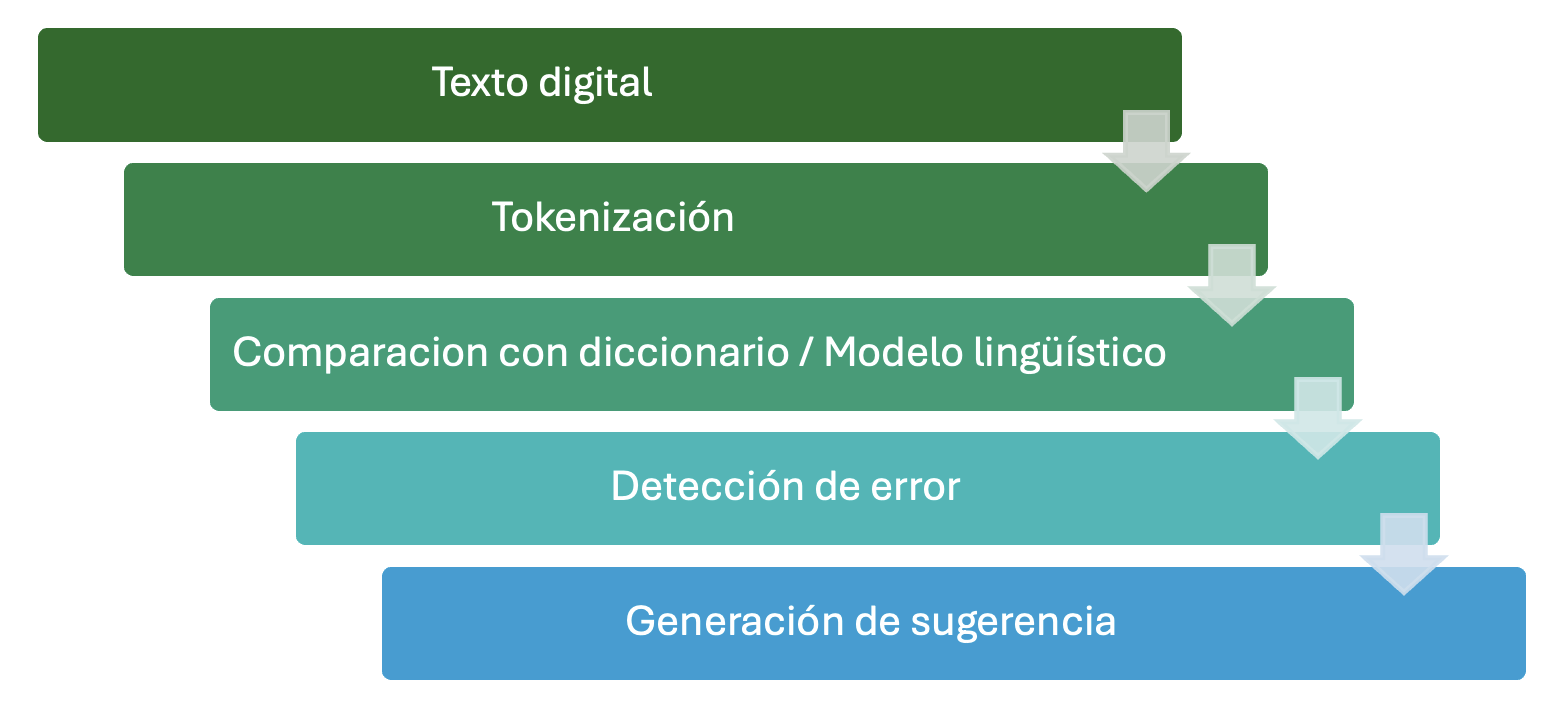
\includegraphics[width=0.7\textwidth]{Imagenes/procesoNLP.png}
    \caption{Flujo básico del proceso de corrección ortográfica mediante NLP. Elaboración con base en \cite{jurafsky2023speech}}
    \label{fig:NLP}
\end{figure}


Como se muestra en la Figura \ref{fig:NLP}, el procedimiento inicia con el texto digital previamente obtenido. Posteriormente, en la etapa de tokenización, el sistema divide el texto en unidades mínimas, generalmente palabras o tokens individuales, lo cual facilita su análisis individual y contextual dentro de la oración.

En la siguiente fase, cada token es comparado con un diccionario léxico o modelo lingüístico entrenado. Si una palabra no coincide con las entradas válidas, el sistema la identifica como posible error ortográfico. Para generar una sugerencia, pueden emplearse algoritmos de similitud como la distancia de Levenshtein o modelos estadísticos que calculan la probabilidad de ocurrencia de una palabra dentro de un contexto determinado \cite{jurafsky2023speech}. Este tipo de técnicas permite no solo detectar errores, sino también proponer alternativas adecuadas.

Este enfoque permite ofrecer retroalimentación automatizada en forma de sugerencias, lo cual resulta útil en entornos educativos cuando se busca apoyar el aprendizaje sin reemplazar la intervención del docente. No obstante, la precisión del sistema depende de la calidad del modelo lingüístico, del contexto del texto y de la claridad del contenido procesado.

La integración de NLP dentro del sistema propuesto permite complementar el análisis realizado por el OCR, cerrando el ciclo de procesamiento desde la captura del texto manuscrito hasta la generación de sugerencias ortográficas. Esta integración representa un enfoque más completo para el tratamiento de la información, combinando procesamiento visual y análisis lingüístico.

En los últimos años, el NLP ha experimentado avances significativos gracias al uso de modelos de representación distribuida del lenguaje, conocidos como embeddings, los cuales permiten capturar relaciones semánticas entre palabras en espacios vectoriales de alta dimensión. Estos modelos han demostrado ser efectivos para mejorar tareas de análisis lingüístico, incluyendo la corrección ortográfica contextual y la detección de errores en textos escritos \cite{ref34}.

Asimismo, el uso de modelos más avanzados basados en arquitecturas modernas ha permitido mejorar la comprensión del contexto dentro de una oración, lo que resulta especialmente útil en aplicaciones educativas donde los errores pueden depender no solo de la forma de la palabra, sino de su uso dentro de una estructura gramatical. Esto permite generar sugerencias más precisas y adaptadas al contexto real del usuario.

\subsection{Evaluación del trazo manuscrito}

El trazo manuscrito constituye un elemento relevante dentro del proceso de adquisición de la escritura en educación primaria. La legibilidad de un texto no depende únicamente de la ortografía correcta, sino también de factores visuales y espaciales que permiten interpretar adecuadamente el contenido escrito \cite{mikolov2013distributed, goodfellow2016deep}. Entre estos factores se encuentran la alineación sobre la línea base, la proporción del tamaño de las letras, el espaciado entre palabras y la uniformidad del trazo, los cuales influyen directamente en la claridad y comprensión del texto.

Diversos estudios sobre desarrollo de la escritura señalan que la evaluación de la letra manuscrita puede abordarse mediante parámetros observables que permitan identificar patrones de mejora o dificultad en los estudiantes \cite{berninger2010teaching, graham2010handwriting}. En contextos educativos tradicionales, esta evaluación es realizada por el docente de forma visual y cualitativa; sin embargo, con el apoyo de herramientas digitales es posible establecer métricas básicas que complementen dicha valoración, aportando un enfoque más objetivo al análisis del desempeño.

Desde una perspectiva computacional, algunos de estos parámetros pueden aproximarse mediante técnicas de análisis de imagen, tales como la medición de altura promedio de caracteres, la variación de inclinación o la separación entre segmentos gráficos \cite{marti2002iam, plamondon2000online}. Estas técnicas permiten cuantificar características del trazo que, de otra forma, serían evaluadas únicamente de manera subjetiva. Si bien estos indicadores no sustituyen la evaluación pedagógica, pueden ofrecer información cuantitativa útil para el seguimiento del progreso del estudiante a lo largo del tiempo.

Los principales parámetros considerados para la evaluación básica del trazo en el presente proyecto se describen en la Tabla \ref{tab:parametros_evaluacion}, donde se establecen tanto los criterios pedagógicos como sus posibles aproximaciones computacionales, permitiendo vincular la evaluación tradicional con el análisis automatizado.

\begin{table}[H]
\centering
\caption{Parámetros de evaluación del trazo manuscrito.}
\label{tab:parametros_evaluacion}
\renewcommand{\arraystretch}{1.5} % Da un poco más de espacio vertical entre las filas
\begin{tabular}{|>{\centering\arraybackslash}m{3cm}|>{\centering\arraybackslash}m{5.5cm}|>{\centering\arraybackslash}m{6cm}|}
\hline
\textbf{Parámetro} & \textbf{Descripción} & \textbf{Posible aproximación computacional} \\ \hline
Legibilidad & Claridad visual de los caracteres & Porcentaje de reconocimiento correcto por OCR \\ \hline
Alineación & Ubicación uniforme sobre línea base & Desviación vertical promedio \\ \hline
Tamaño & Proporción consistente de las letras & Altura media de caracteres \\ \hline
Espaciado & Separación adecuada entre letras & Distancia promedio entre segmentos \\ \hline
Uniformidad & Consistencia en forma y grosor del trazo & Variación en contornos detectados \\ \hline
\end{tabular}
\end{table}

Como se observa en la Tabla \ref{tab:parametros_evaluacion}, los parámetros seleccionados combinan criterios pedagógicos tradicionales con posibles métricas de análisis digital. Esta integración permite establecer un modelo básico de evaluación que apoye el seguimiento del desempeño del estudiante sin reemplazar la interpretación docente, sino más bien complementándola.

La incorporación de estos indicadores dentro del sistema propuesto busca complementar el análisis ortográfico realizado mediante NLP, ofreciendo una visión más integral del proceso de escritura. De esta manera, el sistema no solo evalúa la corrección del texto, sino también la calidad del trazo manuscrito, integrando así componentes visuales y lingüísticos dentro de una misma solución tecnológica.

\subsection{Arquitectura de la aplicación web}
El desarrollo de aplicaciones web modernas suele estructurarse bajo patrones de diseño que permiten organizar de manera eficiente los componentes del sistema. Uno de los modelos más utilizados es la arquitectura Modelo Vista Controlador(Model-View-Controller, MVC por sus siglas en inglés), la cual divide la aplicación en tres capas principales: modelo, vista y controlador \cite{ref33}.

En la Figura \ref{fig:MVC} se presenta el esquema general de la arquitectura MVC aplicada al sistema propuesto.

\begin{figure}[H]
    \centering
    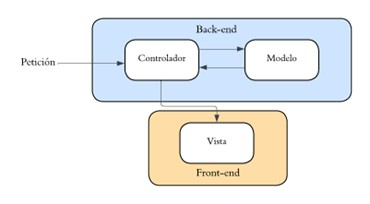
\includegraphics[width=0.7\textwidth]{Imagenes/MVC.jpg}
    \caption{Arquitectura Modelo-Vista-Controlador aplicada al sistema \cite{buschmann1996pattern}.}
    \label{fig:MVC}
\end{figure}

Como se observa en la Figura \ref{fig:MVC}, el flujo de operación inicia con una petición realizada desde el front-end. Esta solicitud es enviada al controlador, ubicado en el back-end, el cual actúa como intermediario entre la interfaz y la lógica del sistema. El controlador procesa la solicitud y se comunica con el modelo, donde se gestionan los datos y la lógica de negocio.

El modelo es responsable del almacenamiento de información, incluyendo usuarios, ejercicios realizados, resultados del OCR, análisis ortográfico mediante NLP y métricas asociadas a la calidad del trazo. Esta separación permite mantener organizada la lógica interna del sistema y facilita futuras modificaciones o ampliaciones.

Posteriormente, el controlador recibe la información procesada y genera una respuesta que es enviada a la vista, encargada de mostrar al usuario la retroalimentación correspondiente. Esta estructura modular favorece la mantenibilidad, escalabilidad y claridad del sistema \cite{ref37}.

Además, el despliegue del sistema en un servidor web funcional permite su acceso mediante navegador, garantizando un entorno controlado para la prueba piloto y la centralización de datos. La adopción del modelo MVC facilita la integración coherente de los módulos de OCR, NLP y evaluación del trazo dentro de una arquitectura estructurada.

\subsection{Experiencia de Usuario y Diseño de Interfaces Educativas}

El diseño de interfaces para aplicaciones educativas destinadas a niños de entre 8 y 10 años requiere un enfoque especializado que considere sus capacidades cognitivas, motoras y de alfabetización en desarrollo \cite{ref38}, \cite{ref39}. La Experiencia de Usuario (UX) en este rango de edad no solo busca la eficiencia en la ejecución de tareas, sino también fomentar el compromiso y minimizar la frustración durante el proceso de aprendizaje \cite{ref38}. Es vital entender que el diseño debe facilitar la transición entre lo digital y lo manual, preservando los beneficios cognitivos que la neurociencia atribuye al trazo físico sobre el teclado \cite{ref40}, \cite{ref41}.

\subsubsection{Consideraciones Cognitivas y Carga Visual}

A diferencia de los usuarios adultos, los estudiantes de tercer y cuarto grado poseen una capacidad limitada para procesar múltiples estímulos simultáneos, por lo que la interfaz debe minimizar la carga cognitiva mediante un diseño limpio y el uso de metáforas visuales claras \cite{ref39}. Esto implica la utilización de áreas de interacción amplias, botones de gran tamaño y tipografías legibles que cumplan con índices de lecturabilidad específicos para su nivel escolar, como el de Fernández-Huerta \cite{ref42}. Un diseño visualmente ordenado permite que el alumno mantenga la atención en el objetivo principal: la práctica de la escritura manuscrita \cite{ref38}.

\subsubsection{Arquitectura de Información y Navegación}
La navegación en sistemas educativos infantiles debe ser sencilla y preferiblemente plana, ya que las estructuras jerárquicas profundas suelen confundir a los usuarios jóvenes \cite{ref38}. Es recomendable que las funcionalidades principales sean accesibles con un mínimo de interacciones y que el uso de íconos representativos esté acompañado de etiquetas de texto sencillas que refuercen la autonomía del estudiante dentro de la plataforma \cite{ref39}. Además, la interfaz de captura debe ser lo suficientemente robusta para generar imágenes de alta calidad que permitan un procesamiento eficiente por parte de arquitecturas avanzadas de reconocimiento de texto como TrOCR \cite{ref43}.

\subsubsection{Retroalimentación y Sistemas de Respuesta}
La retroalimentación inmediata es un componente crítico para el aprendizaje guiado, especialmente en la detección de errores ortográficos y la evaluación de la calidad del trazo \cite{ref38}. El sistema debe proporcionar respuestas multisensoriales que informen al niño sobre sus aciertos y áreas de mejora de manera constructiva, reduciendo la ansiedad ante el error y promoviendo la persistencia en la actividad académica \cite{ref38}. Esta respuesta constante ayuda a consolidar las conexiones neuronales necesarias para el dominio de la escritura \cite{ref40}.

\subsubsection{Engagement y Gamificación}
Para mantener la motivación en tareas que requieren repetición, resulta beneficioso integrar elementos de gamificación como barras de progreso, insignias o recompensas visuales \cite{ref39}. El diseño debe equilibrar estos elementos lúdicos para que actúen como un refuerzo pedagógico efectivo sin convertirse en una distracción del proceso de aprendizaje central \cite{ref39}. El refuerzo positivo mediante herramientas digitales es una estrategia clave para evitar que el estudiante pierda el interés en el desarrollo de sus habilidades caligráficas tradicionales \cite{ref41}.
